\documentclass[a4paper,
			llpt,
			solution,
			accentcolor=tud2d,
			colorbacktitle
			]
			{tudexercise}

\usepackage[utf8]{inputenc}
%\usepackage[ngerman]{babel}
\usepackage{paralist}
\usepackage{amsmath}
\usepackage{pgfplots}
\usepackage{graphicx}
\pgfplotsset{compat=newest}
\usepgfplotslibrary{units}
\usepackage{ziffer} 

\usepackage{multicol} \setlength{\multicolsep}{0pt}

\title{Lösungsvorschlag zur zweiten Hausübung}
\subtitle{Einführung in Net Centric Systems, Sommersemester 2015}
\subsubtitle{Max Weller, Julian Haas, Stefan Pilot}

%\newcommand{\MiBs}{\frac{\mathrm{MiB}}{\mathrm{s}}}
\newcommand{\MiBs}{\,\mathrm{MiB}/\mathrm{s}}

\begin{document}

\maketitle
\section{}


%2.1.txt
\begin{multicols}{2}
\begin{enumerate}

\item
Normalerweise werden bei einem verbindungsorientierten Dienst die Pakete in der Reihenfolge zugestellt, in der sie gesendet wurden. Falls die Pakete in der falschen Reihenfolge beim Empfänger ankommen, werden sie entweder verworfen und später neu angefordert, oder aber gepuffert und in der richtigen Reihenfolge weitergereicht.
Es gibt allerdings Ausnahmen, z.B. das TCP-Urgent-Flag, welches den Empfänger veranlasst, ein Paket vorzuziehen.
\\\\\\
\item
Connectionless:
\begin{compactitem}
\item IP-Telefonie
\item Live-TV-Streaming
(es ist wichtig, dass Pakete mit möglichst geringer Latenz ankommen. Verloren gegangene Pakete sollten nicht wiederholt werden.)
\end{compactitem}
Connection-oriented:
\begin{compactitem}
\item Dateidownload (z.B. FTP)
(Daten müssen in der richtigen Reihenfolge und vollständig ankommen)
\item Web (HTTP)
(Webseiten und Bilder sollten in korrekter Reihenfolge übertragen werden)
\end{compactitem}
\end{enumerate}
\end{multicols}
\section{}
\subsection{}
\begin{enumerate}
\item
\begin{multicols}{2}
Während des 200\,ms langen Burst mit Datenrate $20\MiBs$ empfängt der token bucket 4\,MiB Daten:
\begin{align*}
\text{t}_\text{burst}  \cdot \text{R}_\text{max} &= \text{Datenmenge Burst}
\\
200\mathrm{\,ms} \cdot 20\MiBs &= \mathrm{4\,MiB}
\end{align*}
Für t1 = 125\,ms kann der token bucket die empfangenen Daten mit $\mathrm{R}_{\mathrm{max}} = 20\MiBs$, weiterleiten:
\begin{alignat*}{5}
&\mathrm{B}     &&{}+ \mathrm{R} &&{}\cdot  \mathrm{t}_1 &&{}= \mathrm{R}_{\mathrm{max}} &&{}\cdot  \mathrm{t}_1 \\
& 2\mathrm{\,MiB} &&{}+ 4\MiBs &&{}\cdot   \mathrm{t}_1 &&{}= 20\MiBs &&{}\cdot  \mathrm{t}_1\\
&               &&{}         &&{}      \mathrm{t}_1 &&{}= 0,125\mathrm{s} &&{}
\end{alignat*}
Nach diesen 125\,ms verbleiben noch 1.5\,MiB an zu sendenden Daten:
$$4\mathrm{\,MiB} - \left(0.125\mathrm{s} \cdot 20\MiBs\right) = 1,5 \mathrm{\,MiB}$$
Diese 1.5\,MiB werden dann mit der Rate R = $4\MiBs
$
übertragen. Das dauert 375\,ms:
$$
\frac{1,5 \mathrm{\,MiB}}{ 4 \MiBs} = 375\mathrm{\,ms}
$$
Die bis zur vollen Sekunde verbleibenden 500\,ms reichen, bis sich der token bucket wieder gefüllt hat:
$$
4\MiBs \cdot 500\mathrm{\,ms} = 2\mathrm{\,MiB} = \mathrm{B}
$$
\vfill
\columnbreak
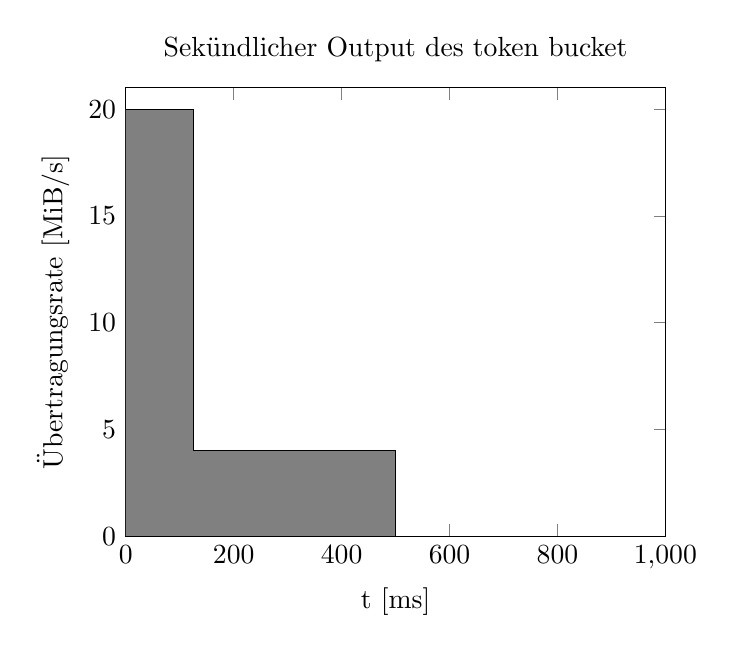
\begin{tikzpicture}
\begin{axis}[title=Sekündlicher Output des token bucket,
			 change x base,
			 x SI prefix=milli,
			 x unit=s,
			 %y SI prefix=mega,
			 xlabel=t,
			 ylabel=Übertragungsrate,
			 y unit=MiB/s,
			 ymin=0,ymax=21,
			 xmax=1,xmin=0,
			 enlargelimits=false]

\addplot[const plot,fill=gray,draw=black]
coordinates {(0,20)(0.125,20)(0.125,4)(0.5,4)(0.5,0)(1,0)}
\closedcycle;
\end{axis}
\end{tikzpicture}
\end{multicols}
\newpage
\item
Während der token bucket Daten mit $20\MiBs$ versendet, füllt sich der leaky bucket mit einer Rate von
$$
20 \MiBs - 10\MiBs = 10\MiBs
$$
Nach den 125\,ms sind
$$
10\MiBs  \cdot 125\mathrm{\,ms} = 1,25 \mathrm{\,MiB}
$$ im leaky bucket.
In den nächsten 375\,ms, in denen der token bucket mit $4\MiBs$ verschickt, leert sich der leaky bucket mit einer Rate von
$$
4\MiBs - 10\MiBs = -6 \MiBs
$$
Die gespeicherten 1,25\,MiB Daten brauchen
$$
\frac{1,25\mathrm{\,MiB}}{6\MiBs} = 208,33\mathrm{\,ms}
$$
um den leaky bucket wieder zu verlassen.
Danach bleibt der leaky bucket bis zur nächsten vollen Sekunde leer.\newline
Antwort: Der leaky bucket verliert keine Daten.
\item
Wie aus den Rechnungen zu b) hervorgeht, lässt sich der Verlauf der Senderate des leaky bucket in vier Phasen aufteilen:
\begin{center}
\begin{tabular}{|c|c|c|c|c|}
\hline
Phase
&
Dauer (ms)
&
Empfangsrate $\left( \MiBs \right)$
&
und Füllrate $\left( \MiBs \right)$
&
Senderate $\left( \MiBs \right)$
\\ \hline
1 & 125    & 20 & 10 & 10 \\ \hline
2 & 208,33 &  4 & -6 & 10 \\ \hline
3 & 166,67 &  4 &  0 &  4 \\ \hline
4 & 500    &  0 &  0 &  0 \\ \hline
\end{tabular}
\end{center}
%Der Graph des sekündlichen Output des leaky bucket sieht also so aus:
\begin{center}
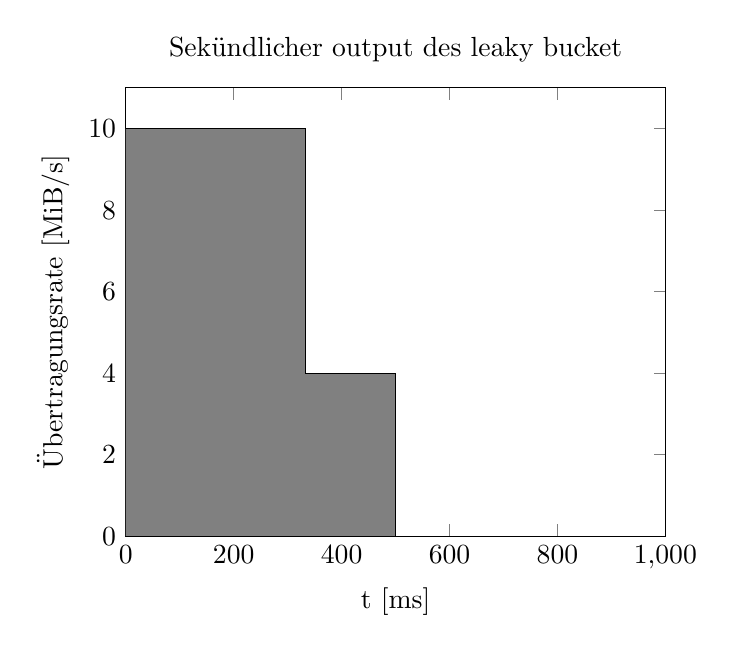
\begin{tikzpicture}
\begin{axis}[title=Sekündlicher output des leaky bucket,
			 change x base,
			 x SI prefix=milli,
			 x unit=s,
			 %y SI prefix=mega,
			 xlabel=t,
			 ylabel=Übertragungsrate,
			 y unit=MiB/s,
			 ymin=0,ymax=11,
			 xmax=1,xmin=0,
			 enlargelimits=false]

\addplot[const plot,fill=gray,draw=black]
coordinates {(0,10)(0.333,10)(0.333,4)(0.5,4)(0.5,0)(1,0)}
\closedcycle;
\end{axis}
\end{tikzpicture}
\end{center}
\end{enumerate}
\subsection{}
\begin{enumerate}
\item
Die Rate, mit der der leaky bucket Daten empfängt, wird hier als $\mathrm{r}_{\mathrm{in}}$ bezeichnet, die in der Übung als $\mathrm{r}$ bezeichnete Outputrate als $\mathrm{r}_{\mathrm{out}}$. Der Füllstand des leaky bucket nach einer der Dauer eines Bursts $\mathrm{t}_\mathrm{burst}$ als $\mathrm{d}_\mathrm{bucket}$. Es gilt:
$$\mathrm{d}_\mathrm{bucket} = \left(\mathrm{r}_\mathrm{in} - \mathrm{r}_\mathrm{out}\right) \cdot \mathrm{t}_\mathrm{burst}$$
$\mathrm{r}_\mathrm{out}$ kann minimal $0\MiBs$ und maximal $2\MiBs$ betragen. Schon durch Einsetzen dieser Randextrema erhält man die Lösung, da $\mathrm{d}_\mathrm{bucket}$ unter 1\,MiB liegt:
\begin{align*}
\mathrm{d}_\mathrm{bucket\,1} = \left(15\MiBs - 0\MiBs\right) \cdot 60\mathrm{\,ms} &= 0,9\mathrm{ \,MiB}\\
\mathrm{d}_\mathrm{bucket\,2} = \left(15\MiBs - 2\MiBs\right) \cdot 60\mathrm{\,ms} &= 0,78\mathrm{\,MiB}
\end{align*}
Antwort: r darf zwischen 0$\MiBs$ und 2$\MiBs$ betragen.
\item
%$$\text{DAS HIER ÜBERPRÜFEN! IST DAS WIRKLICH GEFRAGT?}$$
Bei einem Burst mit $\mathrm{t}_\mathrm{in} = 12\MiBs$ und einer Dauer von 120\,ms läuft der leaky bucket nach 100\,ms über.
\begin{align*}
12 \MiBs - 2 \MiBs \cdot \mathrm{t}_\mathrm{burst} &= 1\,\mathrm{MiB} \\
\mathrm{t}_\mathrm{burst} &= 100\mathrm{\,ms}
\end{align*}
\end{enumerate}
\subsection{}
\begin{enumerate}
\begin{multicols}{2}
\item
Indicate the slots in which the router will decide to\newline send a choke packet with a $= 0,2 $:
$$ \mathrm{u} = 0,2 \cdot \mathrm{u}_\mathrm{prev} + 0,8 \cdot \mathrm{f} $$
\begin{tabular}{|c|c|c|c|}
\hline
t &	f &	$\mathrm{u}_\mathrm{t}$ &	$\mathrm{choke}_\mathrm{t}$	\\ \hline
0 &	0 &	0,000 &				\\ \hline	
1 & 0 &	0,000 &				\\ \hline	
2 &	1 &	0,800 &	X			\\ \hline
3 &	1 &	0,960 &	X			\\ \hline
4 &	1 &	0,992 &	X			\\ \hline
5 &	1 &	0,998 &	X			\\ \hline
6 &	1 &	1,000 &	X			\\ \hline
7 &	0 &	0,200 &				\\ \hline
8 &	1 &	0,840 &	X			\\ \hline
9 &	1 &	0,968 &	X			\\ \hline
\end{tabular}

\item
Indicate the slots in which the router will decide to\newline send a choke packet with a $= 0,8 $:

 $$ \mathrm{u} = 0,2 \cdot \mathrm{u}_{\mathrm{prev}} + 0,8 \cdot \mathrm{f} $$
\begin{tabular}{|c|c|c|c|}
\hline
t &	f &	$\mathrm{u}_\mathrm{t}$ &	$\mathrm{choke}_\mathrm{t}$ \\ \hline
0 &	0 &	0,000 &		\\ \hline	
1 &	0 &	0,000 &	\\ \hline	
2 &	1 &	0,200 &	\\ \hline	
3 &	1 &	0,360 &	\\ \hline	
4 &	1 &	0,488 &	\\ \hline	
5 &	1 &	0,590 &	X\\ \hline	
6 &	1 &	0,672 &	X\\ \hline
7 &	0 &	0,538 &	X\\ \hline	
8 &	1 &	0,630 &	X\\ \hline	
9 &	1 &	0,704 &	X\\ \hline	
\end{tabular}
\end{multicols}
\item
In which of the two previous cases are the reactions of the router to congestion faster? Can this have any drawbacks?
\\
In Fall a erfolgt die Reaktion schneller, da die aktuelle Situation stärker gewichtet ist als die Vergangenheit. 
Dies kann ein Nachteil sein, falls es sich um eine sehr kurze Überlastungssituation handelt, die man eigentlich hätte ignorieren können.
\end{enumerate}
\section{}
\subsection{}
  \begin{center}
    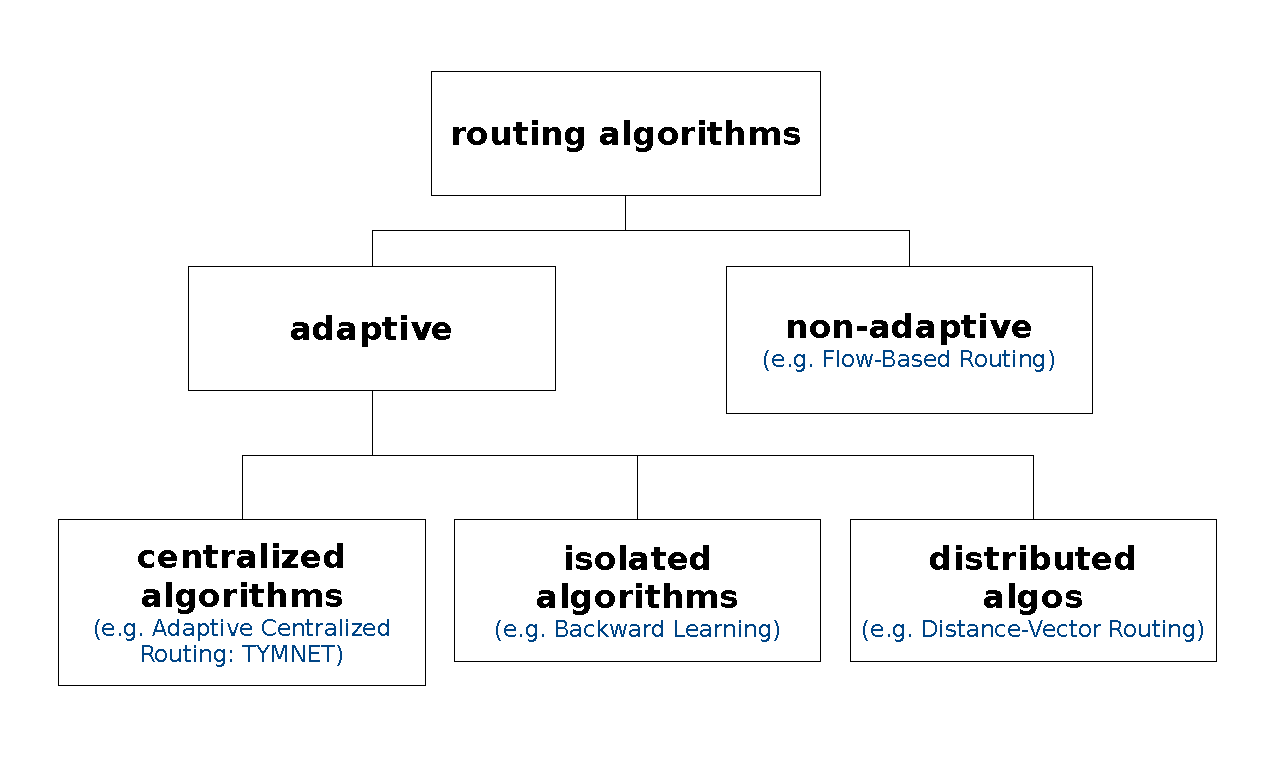
\includegraphics[scale=0.6]{2_3_1.pdf}
  \end{center}

\subsection{}
\begin{center}
\begin{tabular}{|c|c|c|c|c|c|c|}
\hline
Edge i
&
$C_{i} (kbit/sec)$
&
Utilization of path (pkts/sec)
&
$\lambda_{i}(pkts/sec)$
&
$\mu C_{i}(pkts/sec)$
&
$T_{i}(msec/pkt)$
&
Weight
\\ \hline
AB & 30 & 12 & 17 & 60 & 23,26 & 0,2881 \\ \hline
AE & 20 & 6 & 10 & 40 & 33,33 & 0,1695 \\ \hline
BC & 20 & 8 & 12 & 40 & 35,71 & 0,2034 \\ \hline
BD & 10 & 3 & 3 & 20 & 58,82 & 0,0508 \\ \hline
CE & 10 & 5 & 7 & 20 & 76,92 & 0,1186 \\ \hline
DE & 40 & 5 & 10 & 80 & 14,29 & 0,1695 \\ \hline
ABC &   & 4 &    &    &       &\\ \hline
AED &   & 3 &    &    &       &\\ \hline
BAE &   & 1 &    &    &       &\\ \hline
CED &   & 2 &    &    &       &\\ \hline
$\Sigma \lambda _{j}$ & & & 59 & & & \\ \hline
\end{tabular}
\end{center}

\end{document}
